\section{Vorlesung 13}
\begin{definition}[L-periodial]
	$f(x)$ heißt L-periodiel $(L>0)$, wenn gilt : $\forall \in \mathbf{R}: f(x+L)=f(x)$
\end{definition}
\begin{remark}
	Es genügt ,$2\pi$-perodiele Funktionen zu betrachten, denn 
\begin{align*}
f(x) \text{ L-perodial }\Rightarrow  g(x)&= f(x.\frac{L}{2\pi}) ist 2\pi\text{-perodiel, denn }\\
								g(x+2\pi)&= f((x+2\pi).\frac{L}{2\pi})= f(x.\frac{L}{2\pi}+L)=f(x\frac{L}{2\pi})=g(x)\\
f(x)  2\pi-periodiel \ \Rightarrow g(x)&= f(x\frac{2\pi}{L})\text{ ist L-Perodial}\\
\text{wir betrachten nur noch }& 2\pi-periodiele\text{ funktionen}
\end{align*}
\end{remark}
\begin{example}
	$\cos t$ ist $2\pi$-perodiel  
	$\underbrace{\cos(t\frac{2\pi}{\frac{2\pi}{k}})}_{cos(k.t)}$ ist 
	$\overset{\overset{\text{kleinste Periodenlänge}}{\downarrow}}{\frac{2\pi}{k}-}perodiel$ und auch 2$\pi$-perodiel\\
\begin{tikzpicture}
\begin{axis}[
height=5cm,
width=15cm,
axis y line = left,
axis x line = middle,
xticklabels = {$b$,$a$},
ytick       = \empty,
ymin = -2, ymax = 2,
  xmin=0,xmax=4*pi,
xlabel=$t$,
ylabel=$J$,
xtick={0,1.57,3.14,4.71,6.28},
xticklabels={$0$, ,,,$2\pi$}
]
\addplot[domain=0:4*pi,samples=200,blue] {cos(deg(x))}node[above,pos=0.97]{$\cos t$}; 
\end{axis}
\end{tikzpicture}
\end{example}
\begin{remark}
Die Funktionen $\cos(kt)$ und $\sin(kt)$ mit $k\in \{ 0,1,2,... \}   $ sind $2\pi$-periodiel\\ 
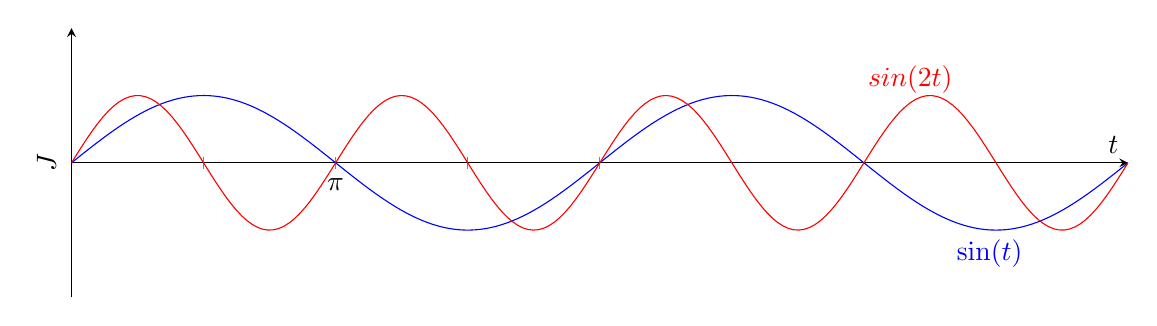
\begin{tikzpicture}
\begin{axis}[
height=5cm,
width=15cm,
axis y line = left,
axis x line = middle,
xticklabels = {$b$,$a$},
ytick       = \empty,
ymin = -2, ymax = 2,
xmin=0,xmax=4*pi,
xlabel=$t$,
ylabel=$J$,
xtick={0,1.57,3.14,4.71,6.28},
xticklabels={$0$, ,$\pi$,,}
]
\addplot[domain=0:4*pi,samples=200,blue] {sin(deg(x))}node[below,pos=0.87]{$\sin(t)$}; 
\addplot[domain=0:4*pi,samples=200,red] {sin(deg(2*x))}node[above,pos=0.80]{$sin(2t)$}; 
\end{axis}
\end{tikzpicture}
\end{remark}
\begin{remark}
$\underbrace{\frac{a_0}{2}.1+\sum_{k=1}^{n}(a_k.cos(k.t)+b_k.\sin(k.t))}_{\text{Trigonomisches Polynom der Ordnung nfalls} a_n \neq 0\text{ oder }b_n \neq 0}$
$a_k$, $b_k$ heißen FOURIER-koeffizienten
\end{remark}
 
	\begin{forest}
	[FOURIER-Theorie 
	[	kontinuierlich[Fourier-Reihen]  ]
	[Diskret [DFT] [FFT]]
	]
\end{forest}\\

\newpage
FOURIER-Synthese\\
gg: $a_k$, $b_k$\\
ges: Trigonomisches Polynom\\
Fourier-Analyse\\
geg: $f(t)$\\
ges: $a_k$, $b_k$ so dass $f(t)$ (!unklar *udsinqieu**** durch ein Trigonomisches Polynom und deren koff. betrachten werden kann)\\
\begin{remark}
$	C[0,2\pi,]$ ist der R-VR der auf $[0,2\pi]$ stetigen Funktionen \\

 \begin{align*}
f,g \in C[0,2\pi] \qquad f \neq g &: t \rightarrow f(t) + g(t)\\
r f &:t \rightarrow rf(t)  (!fehlt)\\
\underbrace{span( \{ 1,\cos t , \cos(2t),\dots,\sin t,\sin (2t),\dots   \}) }_{w}&\text{ ist ein UVR von }  C[0,2\pi]
\end{align*}
\textbf{gegeben:} 
\[ f(x) \in  C[0,2\pi] , 2\pi \quad periodisch   \]
\textbf{gesucht:} \[ f(x) \text{Bestapproximation von } f(x)  \text{ durch ein Element aus W. } \]  
\end{remark}
$\hat{f}(x)$ ist eine Orthogonal-Projektion von $f(x)$ in W. Dazu braucht man eine Orthogonal-Basis von W \\
z.z Die Elemente \{ 1 , cos(t) , cos(2t), ... , sin(t) , sin(2t), ... \} sind paarweise orthogonal.\\
\textbf{Behauptung}\\
Die Vektoren aus der oben erwähnten Mengen sind paarweise orthogonal bezüglich des Skalarprodukt.
Seien f , g stetige Funktionen aus $C[0,2 \pi]$  
\begin{align*}
\Rightarrow f . g := \int_{0}^{2 \pi} {f(t) . g(t) dt } 
\end{align*}


